\documentclass[a4paper,11pt]{report}
\usepackage[utf8x]{inputenc}
\usepackage[portuges,english]{babel}
\usepackage{graphicx}
\usepackage{color}
\definecolor{bordo}{RGB}{192,0,0} %--Cor fancy que eu gosto!
\usepackage{makeidx}
\usepackage{caption}
\usepackage{subcaption}
\usepackage{indentfirst}
\usepackage{verbatim}
\usepackage{amsmath}
\usepackage{graphicx}
\usepackage{setspace}
\newcommand{\HRule}{\rule{\linewidth}{0.5mm}}
\usepackage{trajan}
\usepackage{fetamont}
\usepackage{duerer}
\usepackage{lmodern}
\usepackage[T1]{fontenc}
\usepackage{mathtools}
\usepackage{graphicx,wrapfig,lipsum}
\usepackage{framed}
\usepackage{capt-of}
\usepackage{gensymb}
\usepackage{mdframed}
\usepackage{xcolor}
\usepackage{tikz}
\usetikzlibrary{calc}
\usepackage{empheq}
\usepackage{nameref} %Para utilizar nameref
\usepackage[makeroom]{cancel}
\usepackage{amssymb} %para poder usar \leqslant no math mode
\usepackage{fancyhdr} %-estilo da pagina
%\usepackage{showframe}
\usepackage[margin=2.5cm]{geometry}
\usepackage[hypertexnames=false]{hyperref}
\usepackage{multirow}
\usepackage{pdfpages}
\usepackage{lscape} %para usar página horizontal
\usepackage{multicol} %para poder por 3 figuras alinhas
\usepackage{cases}


%%% - Caso queira utilizar anexos
\newcommand{\annexname}{Annex}
\makeatletter
\newcommand\annex{\par
  \setcounter{chapter}{0}%
  \setcounter{section}{0}%
  \gdef\@chapapp{\annexname}%
  \gdef\thechapter{\@Roman\c@chapter}}
\makeatother

%%%   Para que os capitulos so tenham o titulo e nao a numeraçao de capitulo%%%%%%
  \usepackage{titlesec}
  \titleformat{\chapter}
  {\Large\bfseries} % format
  {}                % label
  {0pt}             % sep
  {\Huge}           % before-code
  
 
  
\hypersetup{
    pdftitle={Electronica Geral},    % title
    pdfauthor={Afonso Mendes, David Escudeiro, Élio Pereira, Pedro Pinto},     % author
    }



\newcommand{\parallelsum}{\mathbin{\!/\mkern-5mu/\!}} %para usar o simbolo de paralelo em circuitos


%-Poupar papel
%%%%%\setlength{\headheight}{12pt}
%%%%%\setlength{\voffset}{-50pt}
%\setlength{\hoffset}{-72.27pt}
%%%%%\setlength{\textheight}{692pt}
%%%%%\setlength{\footskip}{30pt}
%\setlength{\marginparwidth}{0pt}
%%%%%\setlength{\marginparsep}{0pt}
%%%%%\setlength{\textwidth}{450pt}
%%%%%\setlength{\oddsidemargin}{0pt}
%%%%%\setlength{\evensidemargin}{0pt}
%%%%%\setlength{\marginparsep}{0pt}






%---------------------COMEÇA O DOCUMENTO---------------------%
%---------------------COMEÇA O DOCUMENTO---------------------%
%---------------------COMEÇA O DOCUMENTO---------------------%
%---------------------COMEÇA O DOCUMENTO---------------------%
%---------------------COMEÇA O DOCUMENTO---------------------%

\begin{document}
	\selectlanguage{portuges}
	
 
\begin{titlepage}

	\begin{flushleft}
	
\includegraphics[width=0.6\textwidth]{./logo}~\\[4cm]
	\end{flushleft}

\begin{center}
\begin{spacing}{2}

	\textsc{\LARGE Electrónica Geral}\\[1cm]

\HRule \\[0.4cm]
{ \huge \bfseries Filtros Activos e Osciladores}\\[0.4cm]

\HRule \\[1.5cm]

\end{spacing}

	\vspace{2cm}

	Afonso Mendes, \quad 75398\\
	David Escudeiro \quad 75195\\
	Élio Pereira, \quad 73666\\
	Pedro Pinto, \quad 70696\\
	\vspace{4cm}
	\today 

\end{center}


\end{titlepage}


\addtocontents{toc}{\protect\thispagestyle{empty}} %para nao ter numeraçao de pagina na pagina da ToC
\tableofcontents %put toc in
%\setcounter{secnumdepth}{-2} %para as secçoes nao apresentarem numero no indice
%\cleardoublepage %start new page
\setcounter{page}{1} %reset the page counter
%%-estilo da pagina
%\pagestyle{fancy}
%\renewcommand{\headrulewidth}{2pt} 
%\lhead[Electrónica Geral]{Electrónica Geral}
%\chead[]{}
%\rhead[Filtros Activos e Osciladores]{Filtros Activos e Osciladores}
%\lfoot[]{}
%\cfoot[\thepage]{\thepage}
%\rfoot[]{}


%%%%%%%%%%%%%%%%%%%%%%%%%%%%%%%%%%%%%%%%%%%%%%%%%%%%%%%%%%%%%%%%%%%%%%%%%%%%%%%%%%%%%%%%%%%%%%%%%


\chapter{Secção Biquadrática de Kerwin, Huelsman e Newcomb (KHN)}

Para a análise do circuito neste capítulo optou-se por abordar primeiramente a resposta teórica em frequência do circuito e de seguida a resposta experimental. Depois são analisadas as características do circuito, teórica e experimentalmente com as devidas conclusões.

\section{Funções de transferência a partir do DFS}

\begin{center}
     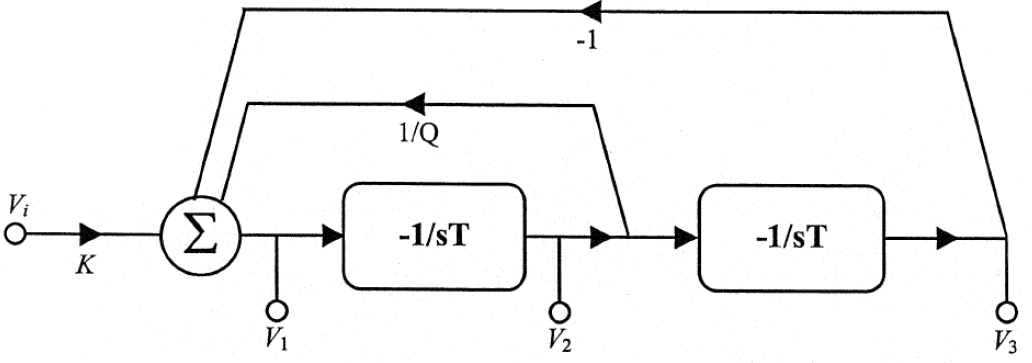
\includegraphics[angle=0,width=0.7\textwidth]{dfskhn.png}
     \captionof{figure}{DFS da secção biquadrática de Kerwin, Huelsman e Newcom (KHN).}
     \label{fig:dfskhn}
     \end{center}

De forma a obter as funções de transferência de cada saída para a entrada do DFS da figura \ref{fig:dfskhn}, determina-se o seguinte sistema, decorrente da análise do mesmo:
\begin{equation*}
\left\{ \begin{matrix*}[l]
 V_1=Kv_i+\dfrac{1}{Q}V_2-V_3\\[0.3cm]
 V_2=\dfrac{-1}{sT}V_1\\[0.4cm]
 V_3=\dfrac{-1}{sT}V_2
\end{matrix*} \right.\Leftrightarrow
\left\{ \begin{matrix*}[l]
 V_1=KV_i+\dfrac{1}{Q}V_2-V_3\\
 V_2=\dfrac{-1}{sT}V_1\\[0.3cm]
 V_3=\Big(\dfrac{-1}{sT}\Big)^2V_1
\end{matrix*} \right.\Leftrightarrow
\left\{ \begin{matrix*}[l]
 V_1=KV_i-\dfrac{w_p}{sQ}V_1-\dfrac{w_p^2}{s^2}V_1\\[0.4cm]
 V_2=\dfrac{-w_p}{s}V_1\\[0.3cm]
 V_3=\dfrac{w_p^2}{s^2}V_1
\end{matrix*} \right.\Leftrightarrow
\end{equation*}
\begin{equation*}
\Leftrightarrow\left\{ \begin{matrix*}[l]
 V_1\bigg(1+\dfrac{w_p}{sQ}+\dfrac{w_p^2}{s^2}\bigg)=KV_i\\[0.4cm]
 V_2=\dfrac{-w_p}{s}V_1\\[0.3cm]
 V_3=\dfrac{w_p^2}{s^2}V_1
\end{matrix*} \right.\Leftrightarrow
\left\{ \begin{matrix*}[l]
 \dfrac{V_1}{V_i}=\dfrac{K}{1+\frac{w_p}{sQ}+\frac{w_p^2}{s^2}}\\[0.5cm]
 V_2=-\dfrac{w_p}{s}V_1\\[0.3cm]
 V_3=\dfrac{w_p^2}{s^2}V_1
\end{matrix*} \right.\Leftrightarrow
\end{equation*}

\begin{equation} \label{eq:ftDFSKHN}
\Leftrightarrow\left\{ \begin{matrix*}[l]
 T_1=\dfrac{V_1}{V_i}=\dfrac{Ks^2}{s^2+\frac{w_p}{Q}s+w_p^2}\\[0.5cm]
 T_2=\dfrac{V_2}{V_i}=-\dfrac{Kw_ps}{s^2+\frac{w_p}{Q}s+w_p^2}\\[0.5cm]
 T_3=\dfrac{V_3}{V_i}=\dfrac{Kw_p^2}{s^2+\frac{w_p}{Q}s+w_p^2}
 \end{matrix*} \right.
\end{equation}\\


Relativamente a $T_1$, a resposta em frequência é característica de um filtro passa-alto, pois atenua os valores para frequências baixas, $\omega\approx 0$, e deixa passar o sinal para frequências elevadas. Isto verifica-se fazendo $\lim_{\omega\to0}T_1(j\omega)=0$ e $\lim_{\omega\to\infty} T_1(j\omega)=K$.



Para a função de transferência $T_2$, o numerador tem um zero em $s=0$ revelando um filtro passa-banda. Tanto as altas e baixas frequências são atenuadas e apenas as frequências perto de $\omega_p$ é que passam, ou seja, $\lim_{\omega\to 0}T_2(j\omega)=0$ e $\lim_{\omega\to\infty}T_2(j\omega)=0$. Quanto à banda passante é centrada em $w_p$ (que se deduz calculando $\frac{dT_2}{ds}=0\Rightarrow s=w_p$) e $\lim_{\omega\to w_p}|T_2(j\omega)|=KQ$.

Por último, $T_3$ é um filtro passa baixo. Atenua as altas frequências e deixa passar as baixas frequências como se pode verificar por $\lim_{\omega\to 0}T_3(j\omega)=K$ e $\lim_{\omega\to\infty}T_3(j\omega)=0$.

Para as três funções de transferência verifica-se que o denominador é igual $(s^2+\dfrac{w_p}{Q}s+w_p^2)$ e os pólos são $\Bigg(s\pm\frac{\sqrt{-(4Q^2-1)w_p^2}-w_p}{2Q}\Bigg)$.

\section{Análise do Circuito}
\begin{center}
     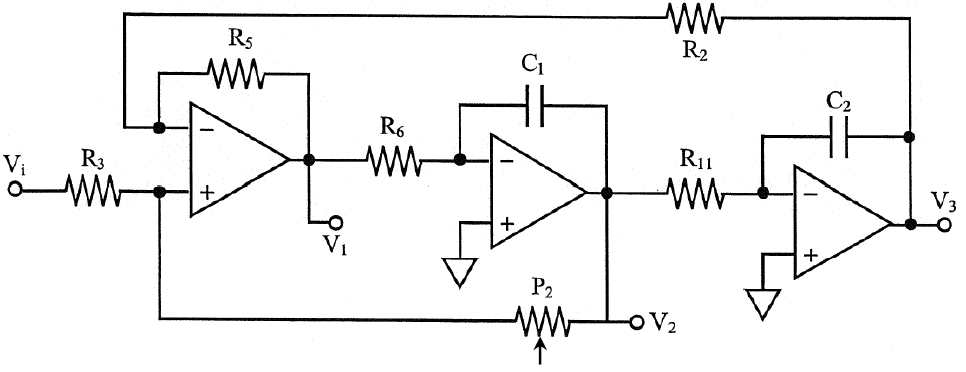
\includegraphics[angle=0,width=0.9\textwidth]{khn.png}
     \captionof{figure}{Secção biquadrática de Kerwin, Huelsman e Newcom (KHN).}
     \label{fig:khn}
     \end{center}
     
Analisando o circuito da figura \ref{fig:khn}, note-se que à entrada se tem um circuito de diferença com a particularidade de que no terminal de entrada positivo a resistência $P_2$ não está ligada à massa mas sim à entrada $V_2$. Por essa razão, não é possível utilizar a expressão deduzida nos slides das aulas teóricas para a tensão de saída de um circuito de diferença e iremos, então, aplicar as leis de Kirchhoff ao circuito de forma a chegar à relação desejada.

\begin{center}
     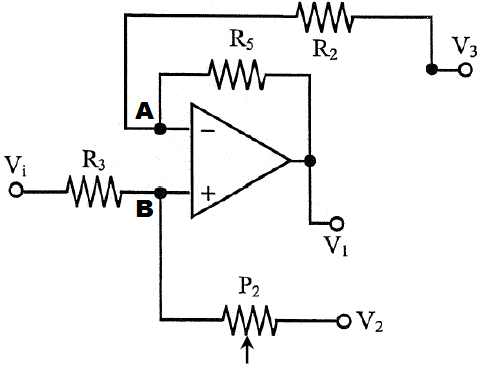
\includegraphics[angle=0,width=0.5\textwidth]{cdif.png}
     \captionof{figure}{Sub-sircuito elementar de diferença.}
     \label{fig:cdif}
     \end{center}


Assumindo o amplificador operacional ideal, as impedâncias de entrada consideram-se infinitas e o ganho do amplificador também infinito. Daqui resulta:
\begin{equation} \label{eq:ampopideal}
\left\{ \begin{matrix*}[l]
	V^+=V^-\Leftrightarrow V_B=V_A\\
	I^+=I^-=0
	\end{matrix*} \right.
\end{equation}

Ora, aplicando a lei dos nós
\begin{itemize}
\item 
$\frac{V_A-V_1}{R_5}=\frac{V_3-V_A}{R_2}\Leftrightarrow V_A=\dfrac{R_5V_3+R_2V_1}{R_5+R_2}$
\item
$\frac{V_i-V_B}{R_3}=\frac{V_B-V_2}{P_2}\Leftrightarrow V_B=\dfrac{P_2V_i+R_3V_2}{R_3+P_2}$
\end{itemize}

Fazendo então $V_A=V_B$:

\begin{equation*}
(R_3+P_2)[R_5V_3+R_2V_1]=(R_5+R_2)[P_2V_i+R_3V_2]\Leftrightarrow
\end{equation*}

\begin{equation}\label{eq:v1}
\Leftrightarrow V_1=(P_2V_i+R_3V_2)\frac{1}{R_2}\dfrac{R_2+R_5}{R_3+P_2}-\frac{R_5}{R_2}V_3
\end{equation}
	
	

Analisando novamente o esquema inteiro, constata-se que mais à direita se tem um circuito integrador-inversor precedido por outro igual. Com base nos resultados apresentados nos slides das aulas teóricas, podemos então escrever:

\begin{itemize}
\item $\dfrac{V_3}{V_2}=-\dfrac{1}{sC_2R_{11}}$
\item $\dfrac{V_2}{V_1}=-\dfrac{1}{sC_1R_6}$
\item $\dfrac{V_3}{V_1}=\dfrac{V_3}{V_2}\dfrac{V_2}{V_1}=\dfrac{1}{s^2C_1C_2R_6R_{11}}$
\end{itemize}

Resolvendo a equação \ref{eq:v1} em ordem a $V_1/V_i$ e tomando a seguinte simplificação...

\begin{equation*}
A=\dfrac{1}{R_2}\dfrac{R_2+R_5}{R_3+P_2}
\end{equation*}

...deduz-se então

\begin{equation*}
V_1=(P_2V_i+R_3V_2)A-\frac{R_5}{R_2}V_3\Leftrightarrow V_1=P_2AV_i+AR_3V_1\Bigg(-\frac{1}{sC_1R_6}\Bigg)-\frac{R_5}{R_2}\frac{V_1}{s^2C_1C_2R_6R_{11}}\Leftrightarrow
\end{equation*}
\begin{equation*}
V_1\Bigg[1+\frac{R_3A}{sC_1R_6}+\frac{R_5}{R_2}\frac{1}{s^2C_1C_2R_6R_{11}}\Bigg]=V_iP_2A\Leftrightarrow \frac{V_1}{V_i}=\frac{s^2C_1C_2R_6R_{11}P_2A}{s^2C_1C_2R_6R_{11}+sR_3AC_2R_{11}+R_5/R_2}\Leftrightarrow
\end{equation*}
\\
\begin{equation}\label{eq:T1}
\Leftrightarrow\boxed{\dfrac{V_1}{V_i}=\dfrac{s^2P_2A}{s^2+s\frac{R_3A}{C_1R_6}+\frac{R_5}{C_1C_2R_2R_6R_{11}}}=\dfrac{s^2}{s^2+2.1277\times 10^4s+4.527\times 10^8}}
\end{equation}\\

Para deduzir as funções de transferência para $V_2$ e $V_3$ basta voltar atrás e aplicar o que já foi mostrado:
\begin{equation}\label{eq:T2}
\boxed{\dfrac{V_2}{V_i}=\dfrac{V_2}{V_1}\dfrac{V_1}{V_i}=-\dfrac{s\frac{P_2A}{C_1R_6}}{s^2+s\frac{R_3A}{C_1R_6}+\frac{R_5}{C_1C_2R_2R_6R_{11}}}=-\dfrac{2.1277\times 10^4s}{s^2+2.1277\times 10^4s+4.527\times 10^8}}
\end{equation}\\
\begin{equation}\label{eq:T3}
\boxed{\dfrac{V_3}{V_i}=\dfrac{V_3}{V_1}\dfrac{V_1}{V_i}=\dfrac{\frac{P_2A}{C_1C_2R_6R_{11}}}{s^2+s\frac{R_3A}{C_1R_6}+\frac{R_5}{C_1C_2R_2R_6R_{11}}}=\dfrac{4.527\times 10^8}{s^2+2.1277\times 10^4s+4.527\times 10^8}}
\end{equation}

\section{Resultados obtidos e diagramas de Bode}
Durante a sessão laboratorial observou-se cada uma das saídas do circuito (correspondentes a cada um dos filtros) de forma a poder comparar os resultados teóricos com valores experimentais. Após análise dos dados obtidos, é possível sobrepor a informação recolhida experimentalmente nos diagramas de Bode esperados para cada um dos filtros. O tratamento dos dados recolhidos em laboratório foi realizado em \textbf{\emph{Matlab}} consiste nos seguintes passos:
\begin{enumerate}
\item Leitura dos vectores de dados da saída e da entrada do ficheiro \textbf{EXCEL} correspondentes a cada frequência utilizada;
\item Estimação da amplitude de ambos os sinais através da média da diferença entre o máximo e o mínimo de cada vector;
\item Obtenção da magnitude da função de transferência como razão entre as amplitudes estimadas;
\item Conversão da magnitude para dB e do vector das frequências para frequências angulares;
\item Realização do plot em escala semi-logarítmica de $\omega$ para magnitude.
\end{enumerate}
\paragraph{}
A sobreposição dos dados obtidos com as curvas teóricas resulta então nos gráficos seguintes.
\begin{center}
     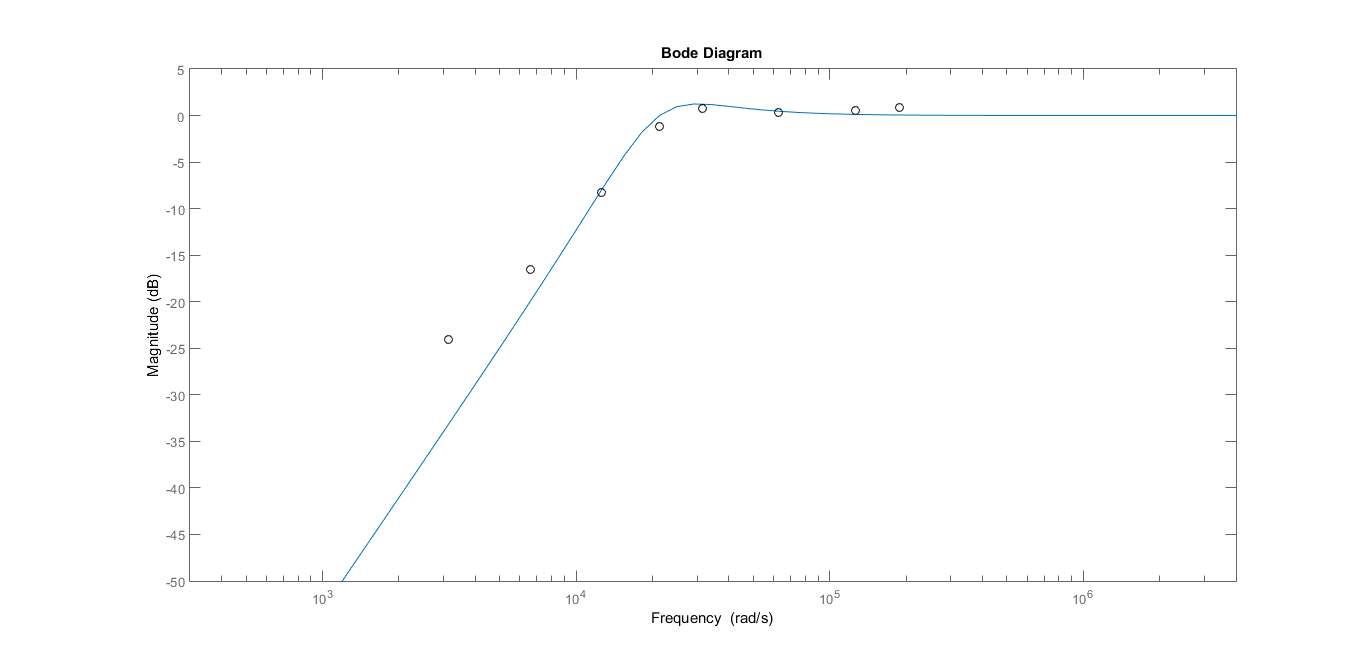
\includegraphics[angle=0,width=0.9\textwidth]{KHNT1exp.png}
     \captionof{figure}{Diagrama de Bode de $T_1$ com pontos experimentais.}
     \label{fig:KHNT1exp}
     \end{center}

\begin{center}
     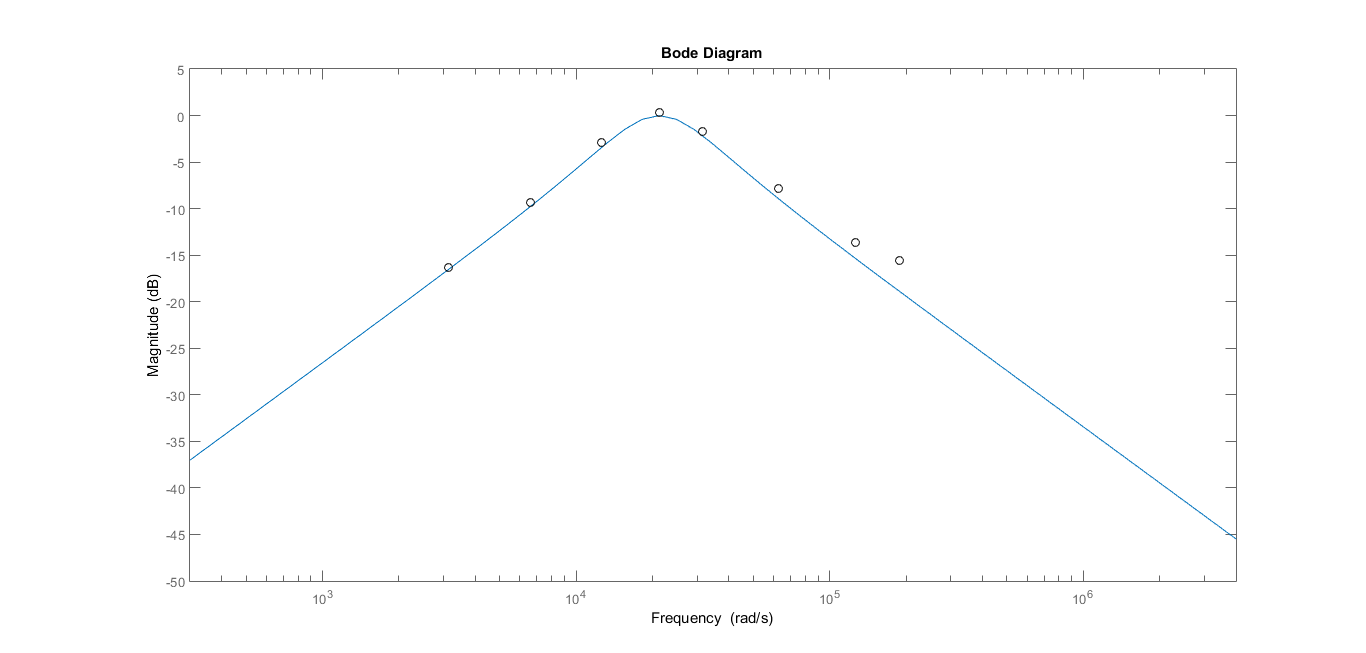
\includegraphics[angle=0,width=0.9\textwidth]{KHNT2exp.png}
     \captionof{figure}{Diagrama de Bode de $T_2$ com pontos experimentais.}
     \label{fig:KHNT2exp}
     \end{center}
     
     \begin{center}
     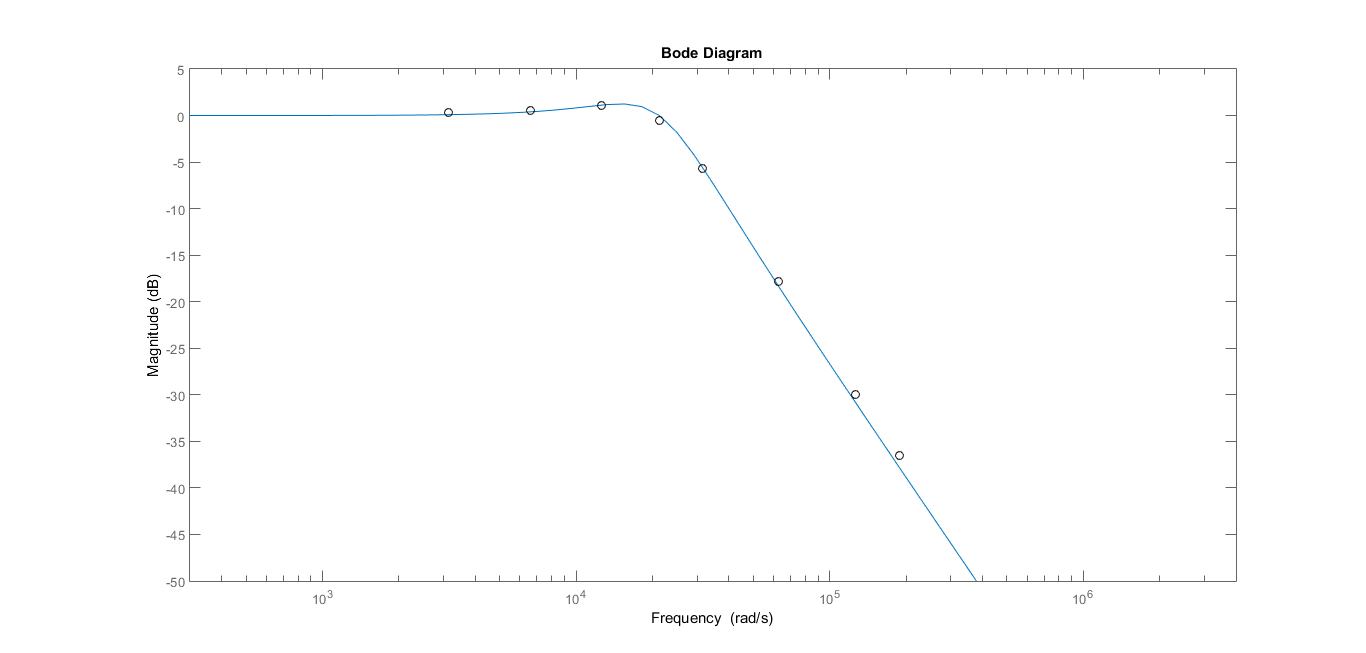
\includegraphics[angle=0,width=0.9\textwidth]{KHNT3exp.png}
     \captionof{figure}{Diagrama de Bode de $T_3$ com pontos experimentais.}
     \label{fig:KHNT3exp}
     \end{center}


É possível concluir que todos as saídas apresentam a característica esperada para o tipo de filtro correspondente.\\
\indent O erro obtido nas duas menores frequências utilizadas na resposta $T1$ pode ser explicado pela sobreposição do ruído de baixas frequências e a grande atenuação do sinal de entrada (filtro passa-alto), o que gera um sinal de saída que, de facto, não se assemelha a uma onda sinusoidal como esperado. As respostas dos outros dois filtros, no entanto, não apresentam tanta atenuação a frequências baixas e, portanto, os pontos experimentais coincidem de forma satisfatória com a previsão teórica.
\section{Valores teóricos e experimentais de $K$, $\omega_p$ e $Q$}

Como esperado após a análise inicial do DFS, o denominador é igual para a três funções de transferência, quando escritas em função dos componentes do circuito. Comparando então os coeficientes do denominador de \ref{eq:T1} com os coeficientes de \ref{eq:ftDFSKHN} e substituindo valores:

\begin{equation} \label{eq:KHNKteorico}
K=P_2A=\frac{P_2}{R_2}\frac{R_2+R_5}{R_3+P_2}=1
\end{equation}

\begin{equation} \label{eq:KHNwpteorico}
\omega_p=\sqrt{\frac{R_5}{C_1C_2R_2R_6R_{11}}}=2.1277\times 10^{4} \quad (\textrm{rad/s})
\end{equation}

\begin{equation} \label{eq:KHNQteorico}
Q=\omega_p\bigg/\bigg(\frac{R_3A}{C_1R_6}\bigg)=\dfrac{R_3+P_2}{R_3}\sqrt{\dfrac{C_1R_2R_5R_6}{C_2R_{11}(R_2+R_5)}}=1
\end{equation}

\begin{table}[h]
\centering
\begin{tabular}{||c|c|c||}
\hline
\textbf{Característica}               & \textbf{Valor teórico} & \textbf{Valor Experimental} \\ \hline\hline
Constante de ganho $K$                & $1$                    & $1.0426$                    \\ \hline
Frequência natural $\omega_p$ (rad/s) & $21277$                & $21830$                     \\ \hline
Factor de qualidade $Q$               & $1$                    & $1.2264$                    \\ \hline
\end{tabular}
\caption{Valores teóricos e experimentais para as características dos filtros.\label{tab:KQwpexperimentais}}
\end{table}

O valor experimental da constante de ganho $K$ é obtido observando o valor do filtro passa-baixo, ou seja, $T_3$, a baixas frequências. Esta conclusão pode ser tirada tomando em consideração a terceira equação do sistema \ref{eq:ftDFSKHN}. Posto isto, utiliza-se como valor de $K$ experimental o valor de $T_3$ obtido na frequência mais baixa utilizada, ou seja, o ponto mais à esquerda na figura \ref{fig:KHNT3exp}. Daqui retiramos então:
\[
\widehat{K}=0.362\,\textrm{dB}=1.0426
\]

Para obter $\omega_p$ e $Q$ necessitamos de um tratamento de dados mais extensivo. Ora, $\omega_p$ corresponde, no diagrama de bode de $T_2$, à frequência de maior ganho e a razão $\omega_p/Q$ corresponde à diferença entre as duas frequências angulares que produzem um ganho inferior em $3\,\textrm{dB}$ ao ganho máximo. Estas relações são apresentadas nos slides das aulas teóricas, de onde se retira o seguinte esquema representativo e onde se tem $a_1=K\,\omega_p$.

     \begin{center}
     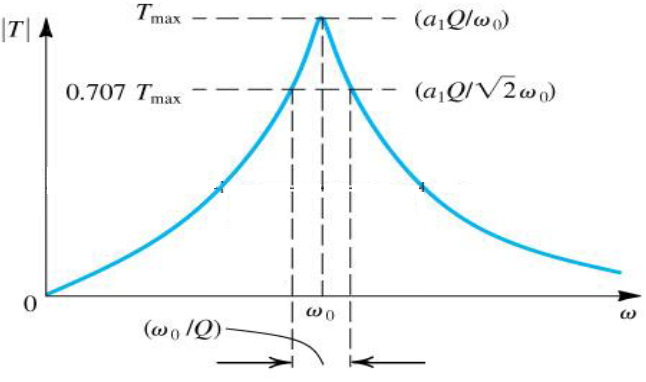
\includegraphics[angle=0,width=0.6\textwidth]{passabanda.png}
     \captionof{figure}{Características do Diagrama de Bode de um Filtro Passa-Banda de segunda ordem.}
     \label{fig:passabanda}
     \end{center}

Como nenhum dos pontos experimentais coincide com o ganho máximo ou com um ganho inferior em $3\,\textrm{dB}$ a esse, decidiu-se fazer uma interpolação por \textit{splines} aos dados obtidos de forma a pode estimar o valor das frequências e dos ganhos nos pontos desejados mas sem ignorar os valores experimentais. Na figura seguinte apresenta-se a curva obtida sobreposta pelos valores que lhe deram origem.

     \begin{center}
     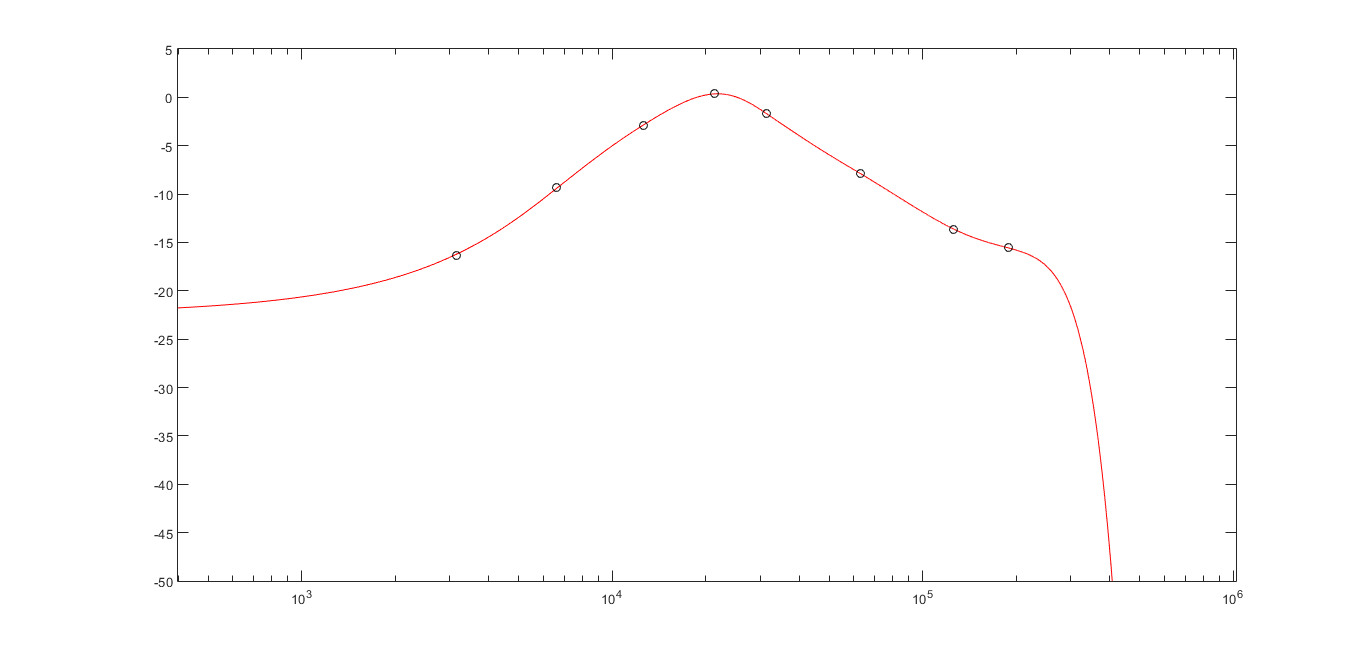
\includegraphics[angle=0,width=0.7\textwidth]{fitbanda.png}
     \captionof{figure}{Interpolação dos valores experimentais do filtro passa-banda ($T_2$).}
     \label{fig:fitbanda}
     \end{center}

É evidente que a curva obtida não apresenta características passa-banda nas baixas frequências. Contudo, para os valores que pretendemos obter não importa o valor dos ganhos nessa gama de frequências. De facto, apenas necessitamos de estimar o comportamento do filtro próximo das frequências utilizadas experimentalmente na banda passante. Analisando então desta forma a curva obtida, basta procurar o seu valor máximo e a frequência angular correspondente para se obter:
\[
\widehat{\omega_p}=2.1830\times 10^4\quad (\textrm{rad/s})
\]

Como já foi explicado, para a obtenção do factor de qualidade apenas necessitamos de encontrar o ponto à esquerda do máximo onde o ganho é inferior em $3\,\textrm{dB}$ e ver a distância $d$ a que está da frequência de ganho máximo. Daqui resulta então:
\[
\widehat{Q}=\frac{\omega_p}{2d}=1.2264
\]

É importante referir que, de facto, a curva obtida por \textit{splines} não apresenta a mesma forma que a esperada na figura \ref{fig:passabanda}. Não só nas altas frequências, como já foi explicado, mas também na banda passante. A razão para tal reside no reduzido número de pontos utilizados na sessão laboratorial. Com um maior número de pontos na banda passante teria sido possível obter uma característica mais realista. Contudo, observamos que os valores obtidos na tabela \ref{tab:KQwpexperimentais} não divergem muito do esperado e, tendo em conta a precisão que era possível obter estes resultados são, pelos motivos explicados, satisfatórios.

\section{Influência do Potenciómetro nas Características do Filtro}

Utilizando o potenciómetro $P_2$ como um divisor de tensão variável, o circuito inicial da figura \ref{fig:khn} altera-se para a configuração apresentada na figura \ref{fig:khn2}

\begin{center}
     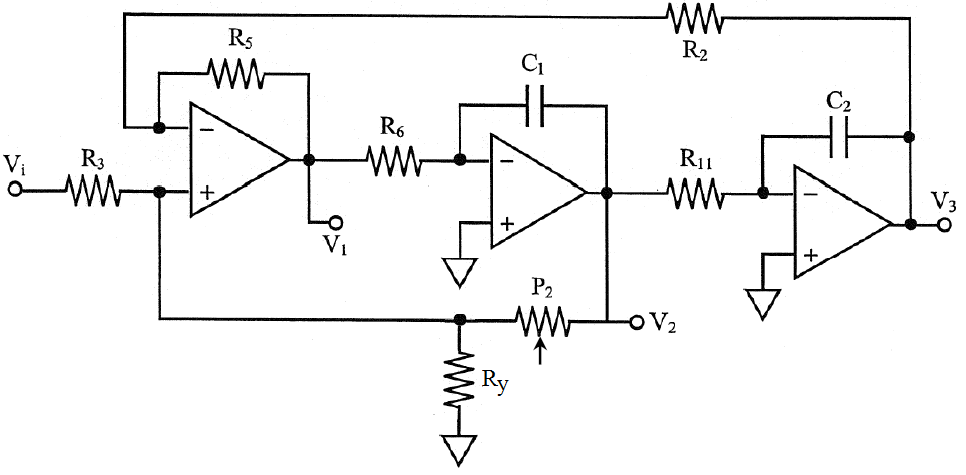
\includegraphics[angle=0,width=0.6\textwidth]{khn2.png}
     \captionof{figure}{Secção KHN com divisor de tensão variável.}
     \label{fig:khn2}
     \end{center}

A alteração face ao circuito inicial implica uma nova análise da função de transferência do primeiro amplificador operacional. De forma a facilitar essa análise, utilizaremos o teorema da sobreposição para os dois casos apresentados na figura seguinte.

\begin{center}
     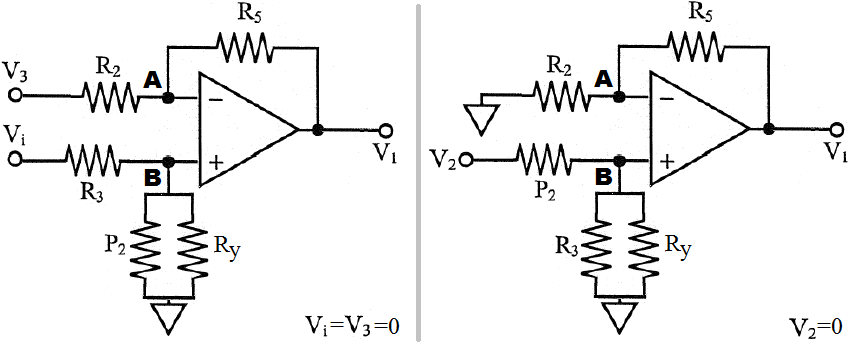
\includegraphics[angle=0,width=0.7\textwidth]{cdifsobreposicao.png}
     \captionof{figure}{Teorema da sobreposição aplicado ao circuito amplificador de diferença.}
     \label{fig:cdifsobreposicao}
     \end{center}

Utilizando a expressão deduzida nos slides das aulas teóricas para o circuito de diferença podemos escrever:

\begin{equation*} 
\left\{ \begin{matrix*}[l]
V_1=\dfrac{R_C}{R_3+R_C}\bigg(1+\dfrac{R_5}{R_2}\bigg)V_i-\dfrac{R_5}{R_2}V_3\quad & , & V_2=0 \\[0.5cm]
V_1=R_B\bigg(1+\dfrac{R_5}{R_2}\bigg)V_2\quad & , & V_i=V_3=0 \\[0.5cm]
 \end{matrix*} \right.
\end{equation*}\\

onde $R_B=\frac{R_3\parallelsum R_y}{P_2+R_3\parallelsum R_y}$, $R_C=P_2\parallelsum R_y$ e $R_A=R_3\parallelsum R_C$. Aplicando o teorema da sobreposição podemos então escrever:

\begin{equation}
V_1=\dfrac{R_A}{R_3}\bigg(1+\dfrac{R_5}{R_2}\bigg)V_i-\dfrac{R_5}{R_2}V_3+R_B\bigg(1+\dfrac{R_5}{R_2}\bigg)V_2
\end{equation}

Escrevendo $V_2$ e $V_3$ como funções de $V_1$ como foi feito anteriormente na análise inicial do circuito, é possível resolver em ordem a $\frac{V_1}{V_i}$ e chegar a:

\begin{equation}
\dfrac{V_1}{V_i}=\dfrac{s^2\frac{R_A(R_2+R_5)}{R_3R_2}}{s^2+s\frac{R_B(R_2+R_5)}{C_1R_2R_6}+\frac{R_5}{C_1C_2R_2R_6R_{11}}}
\end{equation}

Por comparação com a primeira equação do sistema genérico de \ref{eq:ftDFSKHN}, é possível determinar as novas expressões para as características do filtro, substituindo $R_A$, $R_C$ e $R_B$ pelas resistências presentes no circuito.
\begin{equation}
K=\dfrac{R_2+R_5}{R_2}\dfrac{R_A}{R_3}=\dfrac{R_2+R_5}{R_2}\dfrac{R_C}{R_3+R_C}=\dfrac{R_2+R_5}{R_2}\dfrac{P_2(10^4-P_2)}{10^4R_3+P_2(10^4-P_2)}
\end{equation}

\begin{equation}
\omega_p=\sqrt{\dfrac{R_5}{C_1C_2R_2R_6R_{11}}}
\end{equation}

\begin{equation}
Q=\omega_p\;\dfrac{C_1R_2R_6}{R_2+R_5}\;\dfrac{10^4(P_2+R_3)-P_2}{10^4(R_3-P_2)}
\end{equation}

Tendo obtido estas equações é já possível concluir que, para esta montagem, as equações deduzidas anteriormente (\ref{eq:KHNKteorico}, \ref{eq:KHNwpteorico} e \ref{eq:KHNQteorico}) não são válidas para descrever a relação entre o valor das características dos filtros e o valor da resistência $P_2$ do potenciómetro.\\

Com este novo circuito foram medidas, para diferentes valores de $P_2$, as respostas em frequência do filtro passa-banda para frequências próximas da banda passante e do filtro passa-baixo para a frequência de $500\, \textrm{Hz}$, de forma a poder estimar as características dos filtros pelos métodos utilizados anteriormente (interpolação por \textit{splines} para estimar $\omega_p$ e $Q$ e ganho nas baixas frequências para estimar $K$). Apresentam-se de seguida os resultados obtidos após essa análise.


% Please add the following required packages to your document preamble:
% \usepackage{multirow}
\begin{table}[h]
\centering
\label{my-label}
\begin{tabular}{||c|c|c|c|c|c||}
\hline
\multirow{2}{*}{\textbf{Característica}} & \multicolumn{5}{c||}{\textbf{Valor Experimental}}                                                          \\ \cline{2-6} 
                                         & $P_2=2\, k\Omega$ & $P_2=5\, k\Omega$ & $P_2=7.6\, k\Omega$ & $P_2=8.3\, k\Omega$ & $P_2=9.128\, k\Omega$ \\ \hline\hline
Constante de ganho $K$                   & $0.3182$          & $0.4773$          & $0.353$             & $0.294$             & $0.172$               \\ \hline
Frequência natural $\omega_p$ (rad/s)    & $22781$           & $24010$           & $23010$             & $22095$             & $23350$               \\ \hline
Factor de qualidade $Q$                  & $1.1940$          & $1.9909$          & $3.142$             & $4.51$              & $8.32$                \\ \hline
\end{tabular}
\caption{Características do circuito com $P_2$ variável em montagem de divisor de tensão.}
\end{table}





Os resultados obtidos, quando sobrepostos com as curvas teóricas resultantes das equações acabadas de deduzir, apresentam a seguinte característica:

\begin{center}
     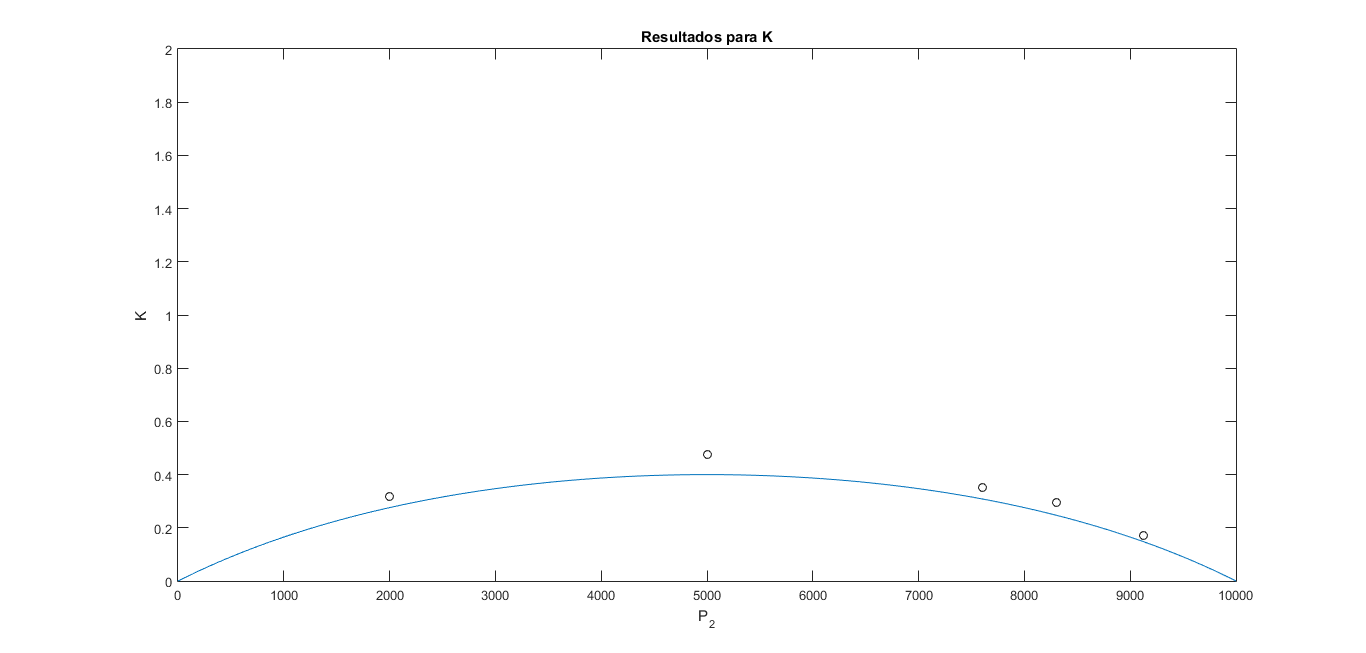
\includegraphics[angle=0,width=0.8\textwidth]{RelacaoKP2KHN.png}
     \captionof{figure}{Relação entre $K$ e $P_2$.}
     \label{fig:RelacaoKP2KHN}
     \end{center}

\begin{center}
     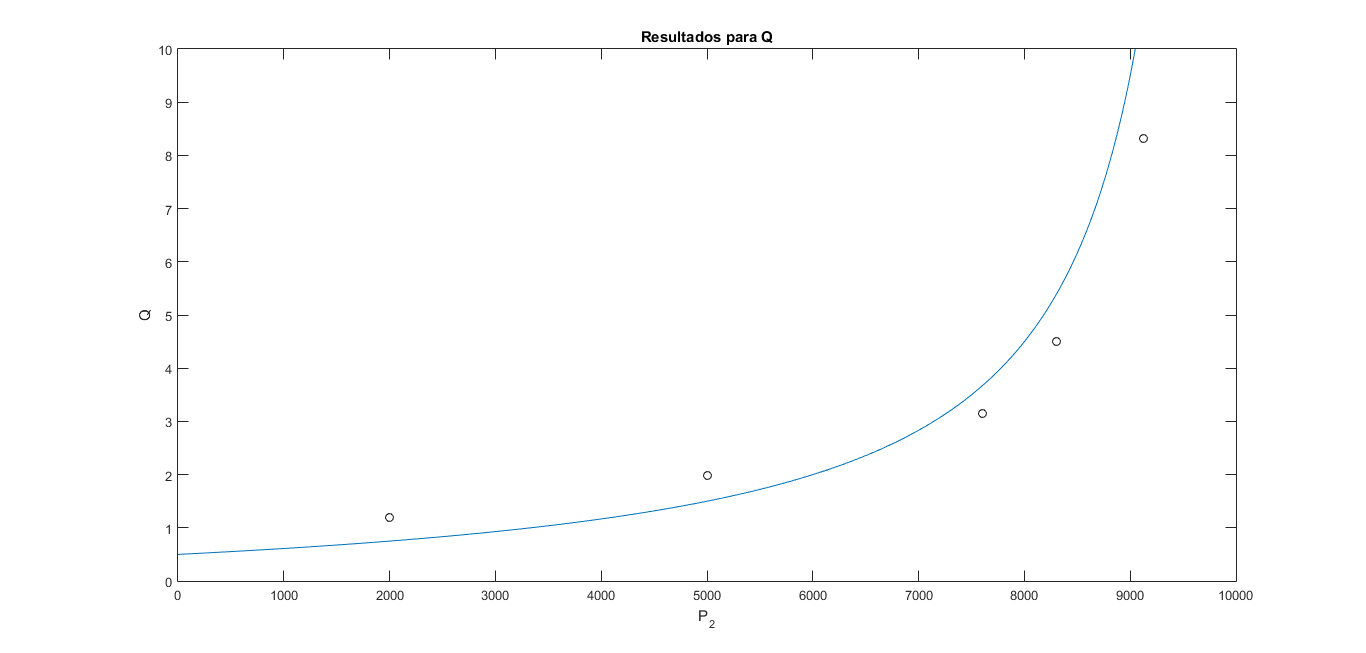
\includegraphics[angle=0,width=0.9\textwidth]{RelacaoQP2KHN.png}
     \captionof{figure}{Relação entre $Q$ e $P_2$.}
     \label{fig:RelacaoQP2KHN}
     \end{center}

\begin{center}
     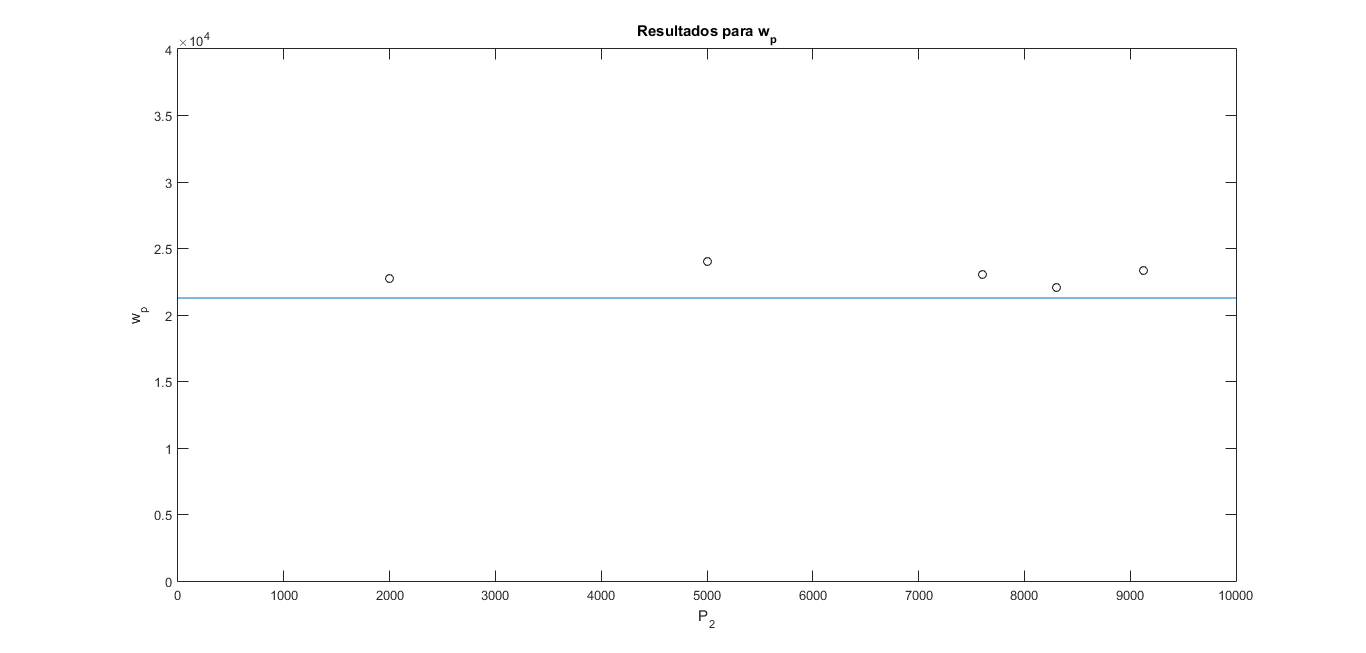
\includegraphics[angle=0,width=0.9\textwidth]{RelacaowpP2KHN.png}
     \captionof{figure}{Relação entre $\omega_p$ e $P_2$.}
     \label{fig:RelacaowpP2KHN}
     \end{center}

Podemos de imediato concluir que $\omega_p$ se mantém aproximadamente constante e igual ao valor esperado na análise inicial. De facto, a expressão obtida para o novo circuito com divisor de tensão para $\omega_p$ é igual à obtida anteriormente e verifica-se, de facto, que o sistema real se comporta como esperado com um erro relativo máximo de $12.85\%$.\\
Quanto a $Q$, os pontos experimentais sugerem que a curva obtida teoricamente descreve razoavelmente bem o comportamento do factor de qualidade quando $P_2$ varia no divisor de tensão. Embora exista um erro relativo que chega a rondar os $35\%$, podemos concluir que a característica dos pontos experimentais comprova um bom ajuste entre a teoria e o sistema real.\\
Por último, a análise comparativa para a constante de ganho $K$ leva-nos a tirar as mesmas conclusões que para os resultados de $Q$. Sendo os erros relativos melhores (próximos dos $20\%$), os resultados permitem concluir que a curva teórica descreve correctamente o filtro real. 



\chapter{Secção biquadrática de Tow-Thomas}



Nesta parte laboratorial pretendemos estudar a secção biquadrática de Tow-Thomas  que se representa pelo seguinte circuito:

  \begin{center}
     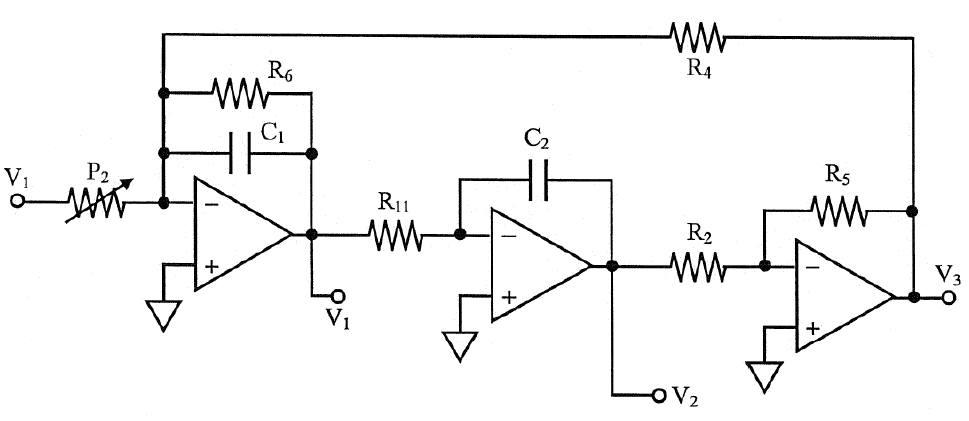
\includegraphics[angle=0,width=0.8\textwidth]{circuito_TT.png}
     \captionof{figure}{Secção biquadrática de Tow-Thomas.}
     \label{fig:circuito_TT}
     \end{center}


\section{Funções de transferência e DFS}


Podemos dividir o circuito da figura \ref{fig:circuito_TT} em 3 sub-circuitos (ver fig. \ref{fig:circuitoselementaresTT}). O primeiro ($\mathcal{A}$) corresponde a um circuito somador-inversor (se considerarmos a impedância equivalente $Z_{eq}=R_6\parallelsum Z_{C_1}$). O segundo ($\mathcal{B}$) corresponde a um circuito integrador-inversor e o terceiro ($\mathcal{C}$) a um circuito multiplicador-inversor.

\begin{multicols}{3}
\begin{center}
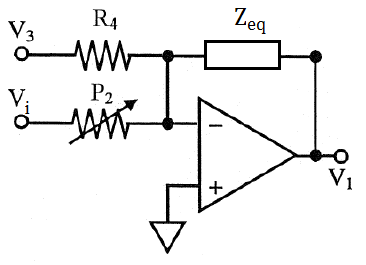
\includegraphics[scale=0.5]{circuito_A.png}
\end{center}
\begin{center}
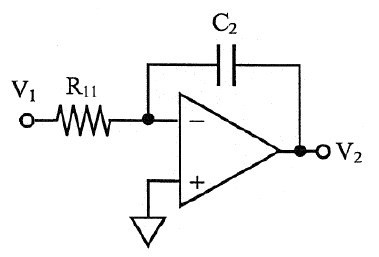
\includegraphics[scale=0.5]{circuito_B.png}
\end{center}
\begin{center}
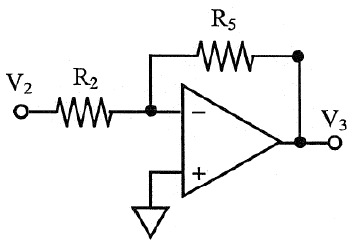
\includegraphics[scale=0.5]{circuito_C.png}
\end{center}
\end{multicols}
 \captionof{figure}{Representação dos 3 sub-circuitos da seccão biquadrática de Tow-Thomas (sub-circuito $\mathcal{A}$ à esquerda , $\mathcal{B}$ ao meio e $\mathcal{C}$ à direita).}
 \label{fig:circuitoselementaresTT}

\paragraph{}De outro ponto de vista, podemos ainda reparar que o circuito $\mathcal{A}$ pode ser dividido em duas unidades separadas: um bloco somador e um bloco integrador inversor amortecido (isto é, com uma alimentação adicional resistiva). Podemos associar (respectivamente) a estes blocos a operação somatório, $\Sigma$ e a operação $-\frac{1}{sT}$ com $T=\frac{1}{\omega_p}$. Tem-se que $R_6$ controla o factor de qualidade do filtro de 2ª ordem, $Q$, o que se exprimirá no diagrama de fluxo de sinal pela operação $\frac{1}{Q}$. Podemos adicionar ao diagrama o ramo de multiplicação de $V_i$ por $K$, sendo $K$ o ganho em DC.

Relativamente ao sub-circuito $\mathcal{B}$, que corresponde a um integrador-inversor, a operação associada a este bloco é $-\frac{1}{sT}$. 

O sub-circuito $\mathcal{C}$ é um multiplicador-inversor com resistências $R_5$ e $R_2$ de igual valor. Logo este bloco é meramente inversor ( operação $-1$).

A secção biquadrática de Tow-Thomas apresenta assim o seguinte diagrama de fluxo de sinal:

 \begin{center}
     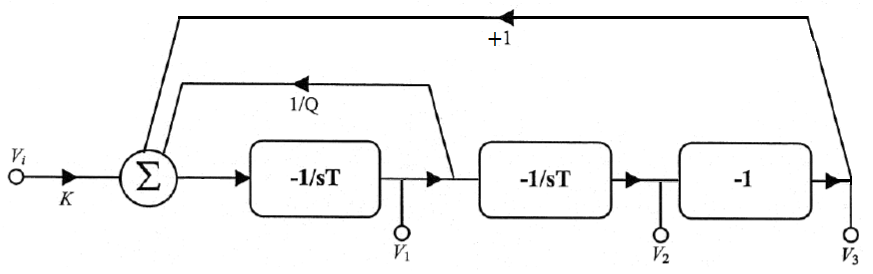
\includegraphics[angle=0,width=0.8\textwidth]{DFS.png}
     \captionof{figure}{Diagrama de fluxo de sinal da secção biquadrática de Tow-Thomas (em que $T=\frac{1}{\omega_p}$)}
     \label{fig:DFS.png}
     \end{center}

A partir da análise das operações representadas no DFS é possível obter as relações entre as tensões em amplitudes complexas $\bar{V}_i$, $\bar{V}_1$, $\bar{V}_2$ e $\bar{V}_3$:


\begin{numcases}
\phantom\bar{V}_1=-\frac{\omega_p}{s}\left(K\bar{V}_i+\frac{1}{Q}\bar{V}_1 +\bar{V}_3\right)\label{eq:TT1}\\
\bar{V}_2=-\frac{\omega_p}{s}\bar{V}_1 \label{eq:TT2}\\
\bar{V}_3=-\bar{V}_2\label{eq:TT3}
\end{numcases}

Substituindo \ref{eq:TT2} em \ref{eq:TT3} e a expressão resultante desta operação em \ref{eq:TT1} vem que:
\begin{numcases}
\phantom\bar{V}_1=-\frac{\omega_p}{s}\left(K\bar{V}_i+\frac{1}{Q}\bar{V}_1 +\frac{\omega_p}{s}\bar{V}_1\right)\label{eq:TT4}\\
\bar{V}_2=-\frac{\omega_p}{s}\bar{V}_1 \label{eq:TT5}\\
\bar{V}_3=\frac{\omega_p}{s}\bar{V}_1 \label{eq:TT6}
\end{numcases}

Desenvolvendo agora apenas \ref{eq:TT4} em ordem a $T_1=\dfrac{\bar{V_1}}{\bar{V}_i}$ tem-se:

$$T_1\left(1+\frac{\omega_p}{Qs}+\frac{\omega_p^2}{s^2}\right)=-\frac{K\omega_p}{s}\Leftrightarrow T_1=-\frac{K\omega_p}{s}\frac{Qs^2}{Qs^2+\omega_ps+\omega_p^2Q}\Leftrightarrow$$

\begin{equation}
\Leftrightarrow T_1=-\dfrac{K\omega_ps}{s^2+\frac{\omega_p}{Q}s+\omega_p^2}\label{eq:TT7}
\end{equation}


Podemos constatar assim, que a função de transferência $T_1$ corresponde à função de transferência de um filtro passa-banda.\\

Por \ref{eq:TT5} e \ref{eq:TT6} obtém-se respectivamente:

\begin{equation}
T_2=\dfrac{K\omega_p^2}{s^2+\frac{\omega_p}{Q}s+\omega_p^2}\label{eq:TT8}
\end{equation}

\begin{equation}
T_3=-\dfrac{K\omega_p^2}{s^2+\frac{\omega_p}{Q}s+\omega_p^2}\label{eq:TT9}
\end{equation}


Portanto, $T_2$ e $T_3$ são funções de transferência respectivas a filtros passa-baixo, sendo que estas são simétricas uma da outra.

É importante referir que $T_1$, $T_2$ e $T_3$ apresentam o mesmo denominador, diferindo apenas no numerador. 

\section{Análise do circuito}

Para determinarmos as constantes $K$, $\omega_p$ e $Q$ podemos começar por analisar o circuito da figura \ref{fig:circuito_TT} e obter as expressões para $T_1$, $T_2$ e $T_3$, agora como funções das resistências e capacidades do circuito. Comparando as novas funções de transferência com as anteriormente obtidas na secção anterior, será então possível extrair as constantes desejadas.\\
As expressões para as relações entre as tensões de saída e de entrada características de cada sub-circuito da figura \ref{fig:circuitoselementaresTT} são:


\begin{numcases}
\phantom\bar{V}_1=-\frac{R_6}{sR_6C_1+1}\left(\frac{\bar{V}_i}{P_2}+\frac{\bar{V}_3}{R_4}\right)\label{eq:TT10}\\
\bar{V}_2=-\frac{1}{sR_{11}C_2}\bar{V}_1 \label{eq:TT11}\\
\bar{V}_3=-\frac{R_5}{R_2}\bar{V}_2 \label{eq:TT12}
\end{numcases}


em que se considerou a impedância equivalente $Z_{eq}=C1\parallelsum R_6=\frac{R_6}{sR_6C_1+1}$.
\\

Para a determinação das funções de transferência basta resolvermos o sistema de equações \ref{eq:TT10}, \ref{eq:TT11} e \ref{eq:TT12} em ordem a $T_1=\dfrac{\bar{V}_1}{\bar{V}_i}$, $T_2=\dfrac{\bar{V}_2}{\bar{V}_i}$ e $T_3=\dfrac{\bar{V}_3}{\bar{V}_i}$.\\

Ora, substituindo \ref{eq:TT11} em \ref{eq:TT12} e a expressão resultante desta operação em \ref{eq:TT10} vem que:

\begin{numcases}
\phantom\bar{V}_1=-\frac{R_6}{sR_6C_1+1}\left(\frac{\bar{V}_i}{P_2}+\frac{R_5}{sR_2R_{4}R_{11}C_2}\bar{V}_1\right)\label{eq:TT13}\\
\bar{V}_2=-\frac{1}{sR_{11}C_2}\bar{V}_1\label{eq:TT14} \\
\bar{V}_3=\frac{R_5}{sR_2R_{11}C_2}\bar{V}_1 \label{eq:TT15}
\end{numcases}


Desenvolvendo agora apenas \ref{eq:TT13}:


$$\bar{V}_1\left(\frac{sR_6C_1+1}{R_6}+\frac{R_5}{sR_2R_4R_{11}C_2}\right)=-\frac{\bar{V}_i}{P_2}\Leftrightarrow \bar{V}_1\left(\frac{s^2R_2R_4R_6R_{11}C_1C_2+sR_2R_4R_{11}C_2+R_5R_6}{sR_2R_4R_6R_{11}C_2}\right)=-\frac{\bar{V}_i}{P_2}$$\\

Isolando $\frac{\bar{V}_1}{\bar{V}_i}$ vem que:

$$T_1=-\frac{sR_2R_4R_6R_{11}C_2}{s^2R_2R_4R_6R_{11}P_2C_1C_2+sR_2R_4R_{11}P_2C_2+R_5R_6P_2}$$\\

Normalizando o coeficiente multiplicativo de $s^2$ no denominador:

\begin{equation}\label{eq:TT16}
\boxed{T_1=-\dfrac{\frac{1}{P_2C_1}s}{s^2+\frac{1}{R_6C_1}s+\frac{R_5}{R_2R_4R_{11}C_1C_2}}=-\dfrac{21.277\times 10^3s}{s^2+21.277\times 10^3s+4.527\times 10^8}}
\end{equation}

Recorrendo a \ref{eq:TT14} e \ref{eq:TT15}:

\begin{equation*}
\boxed{T_2=\dfrac{\frac{1}{P_2R_{11}C_1C_2}}{s^2+\frac{1}{R_6C_1}s+\frac{R_5}{R_2R_4R_{11}C_1C_2}}=\dfrac{4.527\times 10^8}{s^2+21.277\times 10^3s+4.527\times 10^8}}
\end{equation*}

\begin{equation*}
\boxed{T_3=-\dfrac{\frac{R_5}{P_2R_2R_{11}C_1C_2}}{s^2+\frac{1}{R_6C_1}s+\frac{R_5}{R_2R_4R_{11}C_1C_2}}=-\dfrac{4.527\times 10^8}{s^2+21.277\times 10^3s+4.527\times 10^8}}
\end{equation*}


Com $T_1$ determinada, e estando a expressão obtida em função das resistências e capacidades do circuito, será então possível obter as constantes $K$, $\omega_p$ e $Q$ pela comparação desta nova função de transferência com a de \ref{eq:TT7}, de onde resulta:
\begin{equation*} 
\left\{ \begin{matrix*}[l]
\dfrac{\omega_p}{Q}=\dfrac{1}{C_1R_6}\\[0.5cm]
\omega_p^2=\dfrac{R_5}{R_2R_4R_{11}C_1C_2}\\[0.5cm]
K\omega_p=\dfrac{1}{P_2C_1}
 \end{matrix*} \right.
\end{equation*}


Ou seja,
\begin{numcases}
\phantom\omega_p=\sqrt{\frac{R_5}{R_2R_4R_{11}C_1C_2}}=2.1277\times 10^4 \quad\textrm{(rad/s)} \label{eq:TT17}\\
Q=R_6\sqrt{\frac{R_5C_1}{R_2R_4R_{11}C_2}}=1\label{eq:TT18}\\
K=\frac{1}{P_2}\sqrt{\frac{R_2R_4R_{11}C_2}{R_5C_1}}=1 \label{eq:TT19}
\end{numcases}


\section{Resultados obtidos e diagramas de Bode}

\hspace{15pt} Tendo em conta as funções de transferência calculadas anteriormente e utilizando os valores nominais dados no enunciado, pode proceder-se à elaboração dos diagramas de Bode correspondentes às respostas em frequência de cada uma delas.\\

Sendo o denominador comum às três funções de transferência, estas vão ter os mesmos pólos, que se calculam de seguida:
$$s^2+21.277\times10^3 s+4.527\times10^8=0\Leftrightarrow s=\frac{-21.277\times 10^3\pm \sqrt{\left(21.277\times 10^3\right)^2-4\times 1\times 4.527\times 10^8}}{2\times 1}$$

Existem assim dois pólos:

$$
\begin{cases}
s_1=-10.639\times 10^3+j18.426\times 10^3\\
s_2=-10.639\times 10^3-j18.426\times 10^3
\end{cases}
$$

Cujo módulo é: $\left|s_1\right|=21.277\times 10^3 \quad \textrm{rad/s}$

Seguem-se então os diagramas de Bode de amplitude obtidos através das equações descritas anteriormente, sobrepostos pelos pontos experimentais obtidos em laboratório:

\begin{center}
     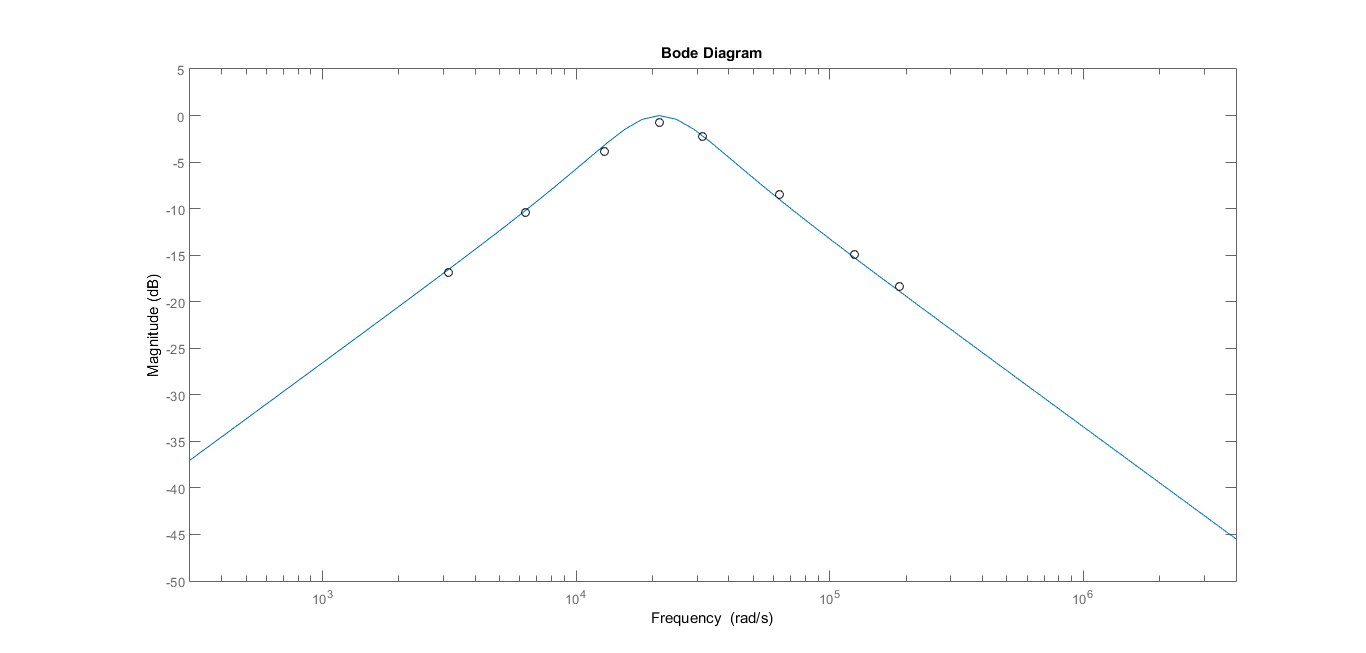
\includegraphics[angle=0,width=0.9\textwidth]{TTT1exp.png}
     \captionof{figure}{Diagrama de Bode de $T_1$ com pontos experimentais.}
     \label{fig:TTT1exp}
     \end{center}

\begin{center}
     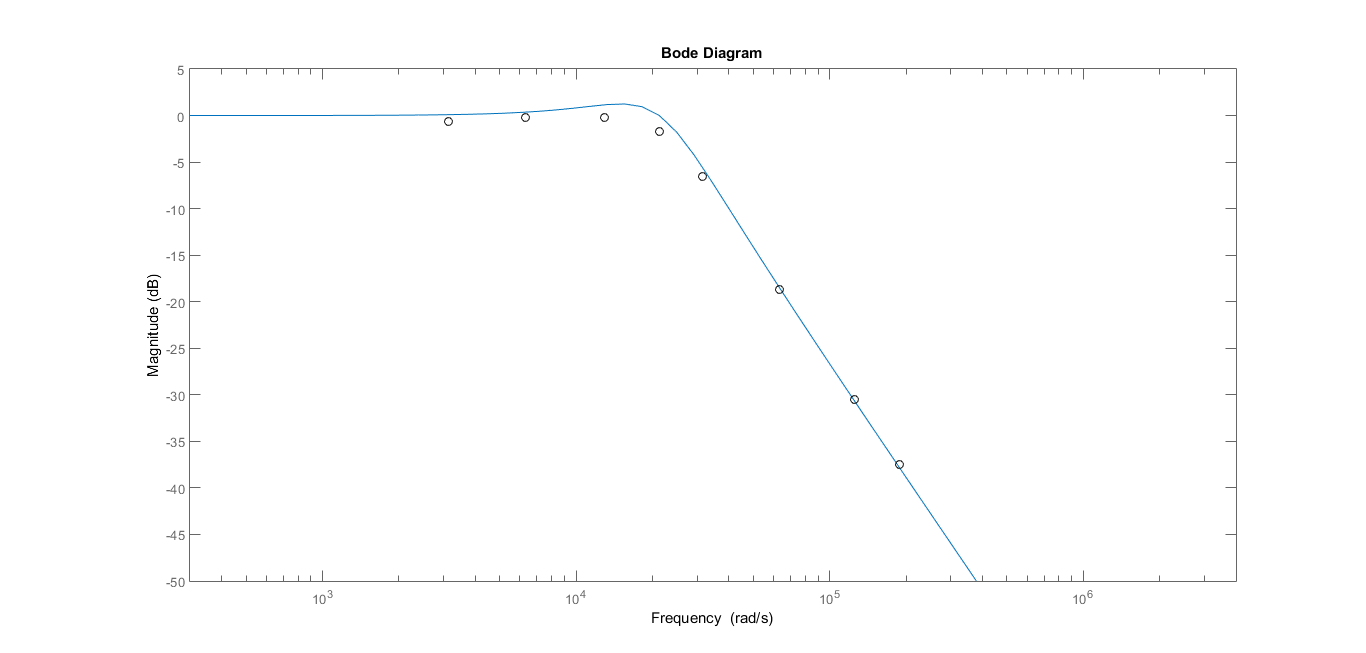
\includegraphics[angle=0,width=0.9\textwidth]{TTT2exp.png}
     \captionof{figure}{Diagrama de Bode de $T_2$ com pontos experimentais.}
     \label{fig:TTT2exp}
     \end{center}
     
 \begin{center}
     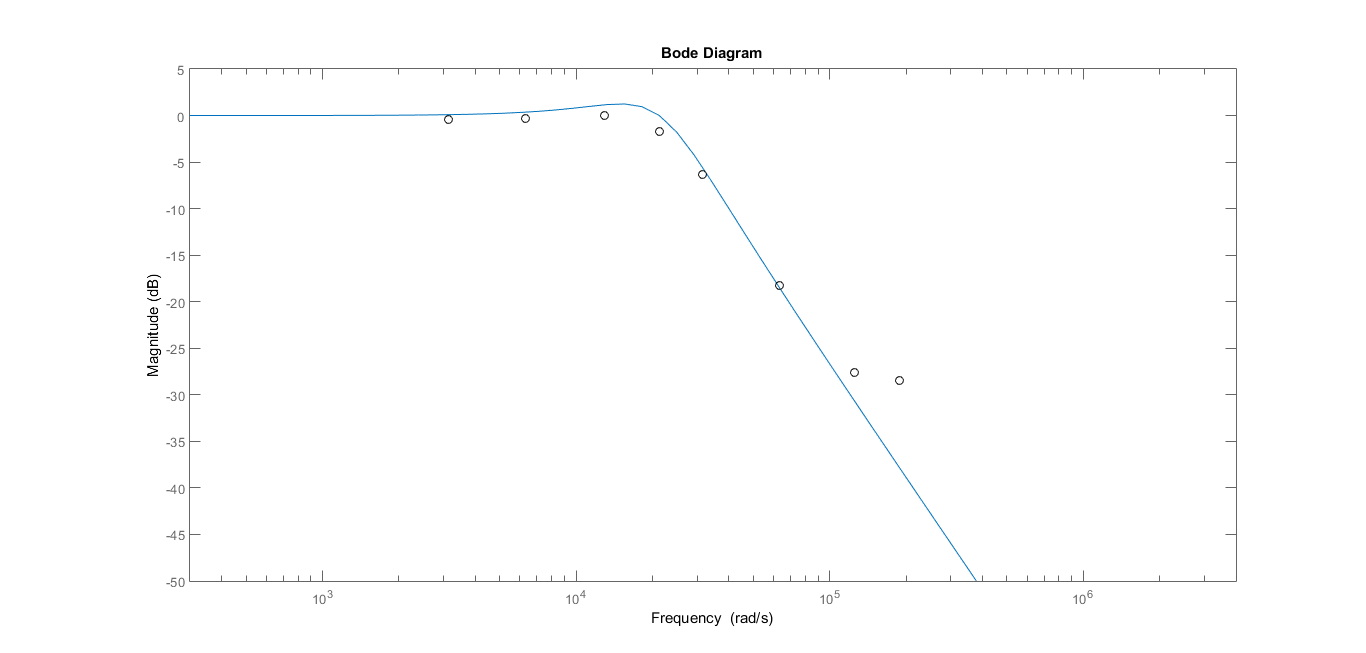
\includegraphics[angle=0,width=0.9\textwidth]{TTT3exp.png}
     \captionof{figure}{Diagrama de Bode de $T_3$ com pontos experimentais.}
     \label{fig:TTT3exp}
     \end{center}


Podemos observar que os diagramas de Bode de magnitude correspondentes às funções de transferência $T_2$ e $T_3$ são iguais em módulo e simétricas, pelo que a única diferença na resposta das duas saídas seria uma oposição de fase de $180\degree$.\\
Verifica-se o comportamento de filtro passa-banda no diagrama correspondente à função $T_1$, bem ajustado pelos pontos experimentais e de filtro passa-baixo nos diagramas correspondentes às funções $T_2$ e $T_3$. Nota-se que os dois últimos pontos experimentais no diagrama de $T_3$ apresentam um erro maior que os correspondentes no diagrama de $T_2$ e, dado que se deveria ter obtido, supostamente, $2$ pares de pontos iguais, conclui-se que esse desvio se deve a uma possível má ligação dos componentes e a um mau contacto que tenha introduzido mais ruído na saída, tendo o erro sido potenciado pelo facto de se estar a trabalhar numa zona da resposta com grande atenuação de sinal.\\
Também se pode observar o efeito do factor derivativo no primeiro diagrama, devido à presença de um zero na origem na função de transferência $T_1$. 

\section{Influência do Potenciómetro nas Características do Filtro}

Recorrendo às equações \ref{eq:TT17}, \ref{eq:TT18} e \ref{eq:TT19} podemos comparar os resultados teóricos com os obtidos experimentalmente para as características dos filtros: $K$, $\omega_p$ e $Q$.

\begin{table}[h]
\centering
\label{tab:TTP2variavel}
\begin{tabular}{||c|c|cccc||}
\hline
\multirow{2}{*}{\textbf{Característica}} & \textbf{Valor}   & \multicolumn{4}{c||}{\textbf{Valor Experimental}}                                 \\ \cline{3-6} 
                          & \textbf{teórico} & $P_2=10\, k\Omega$ & $P_2=5\, k\Omega$ & $P_2=1\, k\Omega$ & $P_2=0.5\, k\Omega$ \\ \hline \hline 
Constante de ganho $K$ em $T_2$          & $1$              & $0.9341$           & $1.9556$          & $10.2326$         & $20.4878$           \\ \hline
Constante de ganho $K$ em $T_3$          & $1$              & $0.9556$           & $2.1333$          & $10.2326$         & $20$                \\ \hline
Frequência natural $\omega_p$ (rad/s)    & $21277$          & $22700$            & $22840$           & $22370$           & $21300$             \\ \hline
Factor de qualidade $Q$                  & $1$              & $1.1860$           & $1.1810$          & $1.1975$          & $1.2007$            \\ \hline
\end{tabular}
\caption {Previsão teórica e observação experimental das características dos filtros activos considerados.}
\end{table}

Tal como para a secção biquadrática KHN, as constantes de ganho $K$ foram estimadas a partir do valor das funções de transferência que representam filtros passa-baixo, $T_2$ e $T_3$, na frequência mais baixa utilizada em laboratório ($500$ Hz).\\
Por sua vez, os valores de $Q$ e de $\omega_p$ foram também estimados da mesma forma que para a secção KHN, ou seja, realizando uma interpolação por \textit{splines} aos pontos experimentais da resposta de $T_1$ de forma a obter uma curva contínua que aproximasse a resposta real obtida em laboratório na gama de frequências utilizada. Tal como anteriormente, os valores de $\omega_p$ e $Q$ são então obtidos com base na figura \ref{fig:passabanda} retirada dos slides das aulas teóricas.\\

Tendo então estimado os valores das características da resposta em frequência de cada filtro variando o valor do potenciómetro $P_2$, procedeu-se à comparação desses resultados com as previsões teóricas descritas pelas equações \ref{eq:TT17}, \ref{eq:TT18} e \ref{eq:TT19} de onde resultam os seguintes gráficos.

\begin{center}
     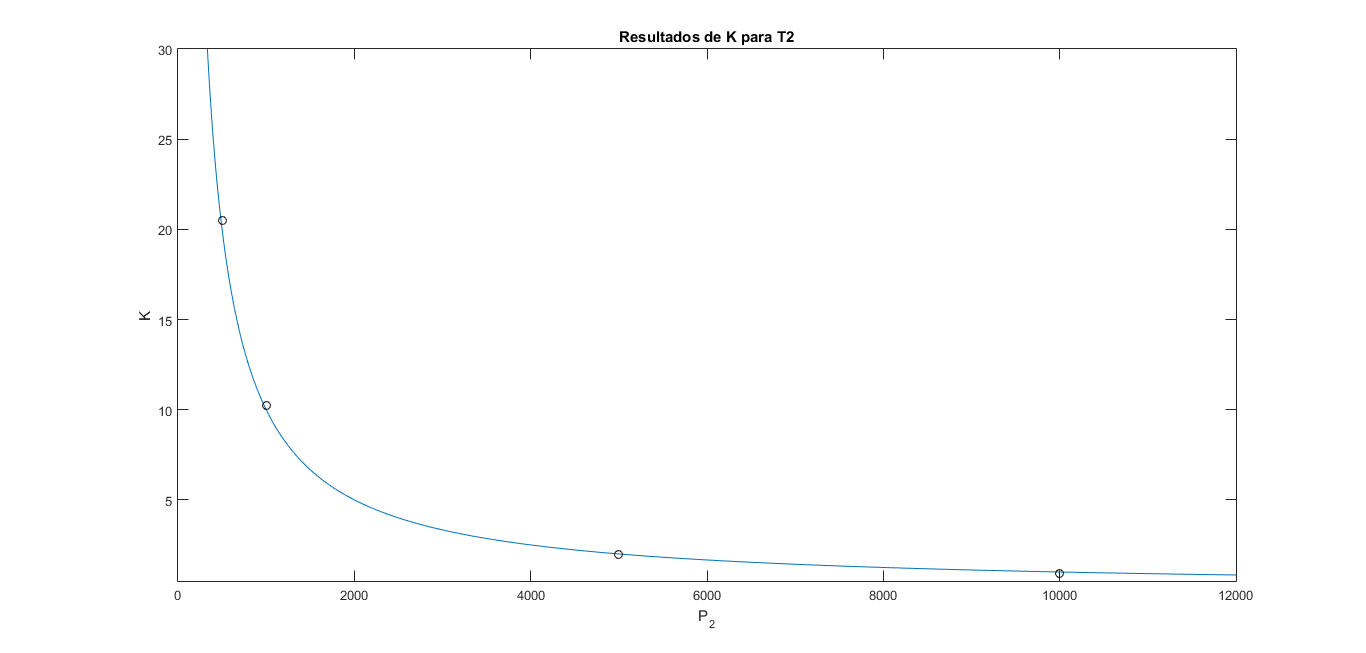
\includegraphics[angle=0,width=1\textwidth]{RelacaoK2P2TT.png}
     \captionof{figure}{Comparação experiência/teoria da relação entre $K$ medido em $T_2$ e o valor de $P_2$.}
     \label{fig:RelacaoK2P2TT}
     \end{center}

\begin{center}
     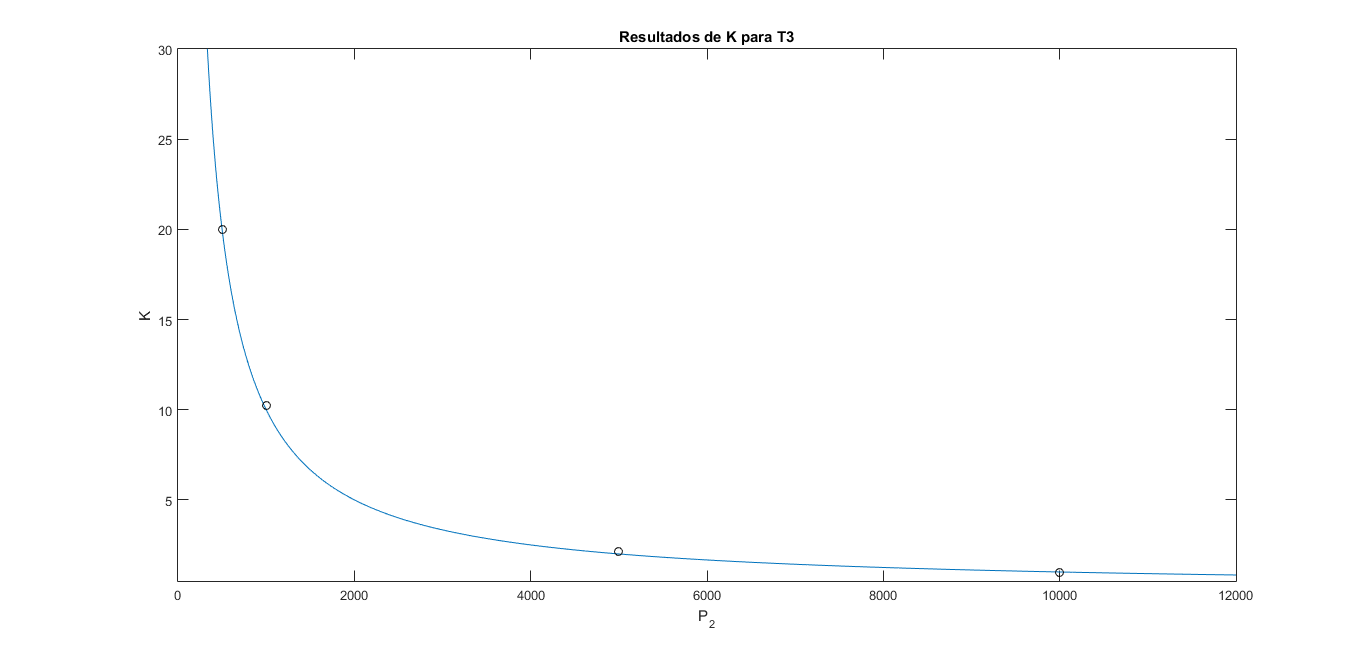
\includegraphics[angle=0,width=1\textwidth]{RelacaoK3P2TT.png}
     \captionof{figure}{Comparação experiência/teoria da relação entre $K$ medido em $T_3$ e o valor de $P_2$.}
     \label{fig:RelacaoK3P2TT}
     \end{center}
     
     Destes dois gráficos podemos tirar a conclusão de que os valores obtidos se ajustam muito satisfatoriamente à curva esperada. Isto não é surpreendente dado que longe das atenuações elevadas os resultados têm sido fiáveis até agora.

\begin{center}
     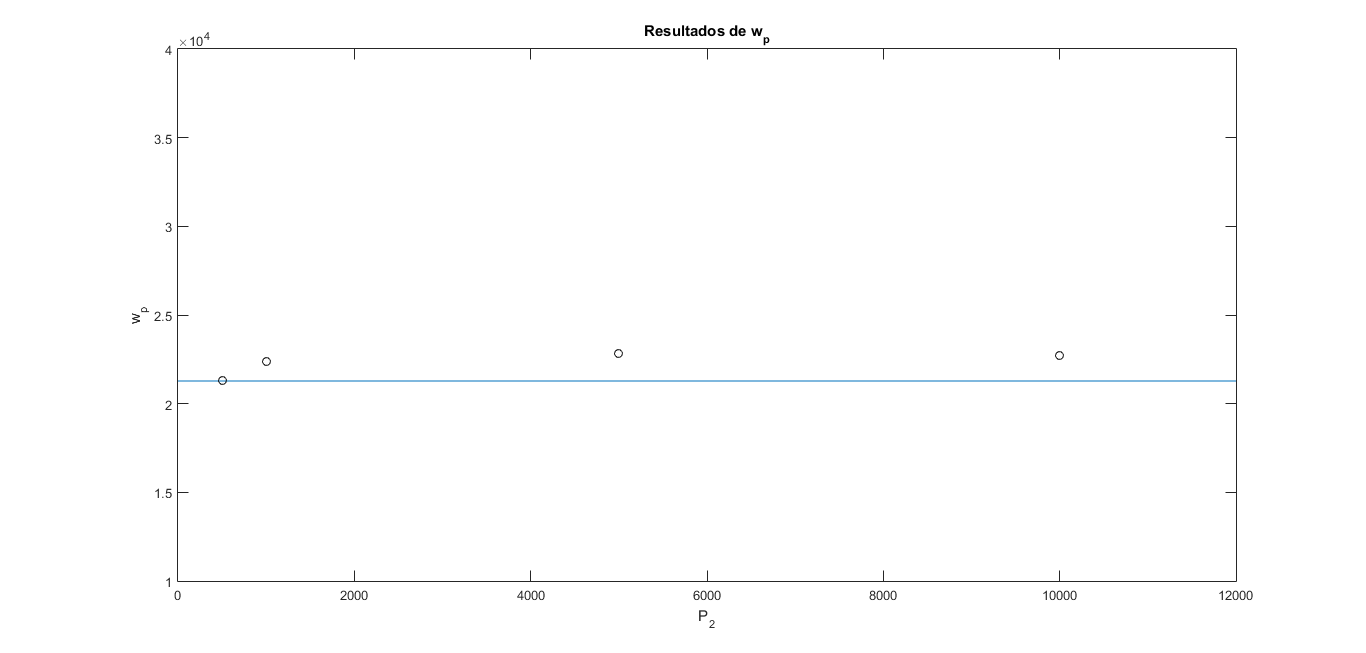
\includegraphics[angle=0,width=1\textwidth]{RelacaowpP2TT.png}
     \captionof{figure}{Comparação experiência/teoria da relação entre $\omega_p$ medido em $T_1$ e o valor de $P_2$.}
     \label{fig:RelacaowpP2TT}
     \end{center}

Relativamente a $\omega_p$, já não é possível confirmar uma óptima concordância entre resultados experimentais e previsão teórica. Contudo, das quatro medições, a que apresenta maior erro relativo é a correspondente a $P_2=5\, k\Omega$ e mesmo nesse caso o erro relativo é de apenas $7.35\%$.

\begin{center}
     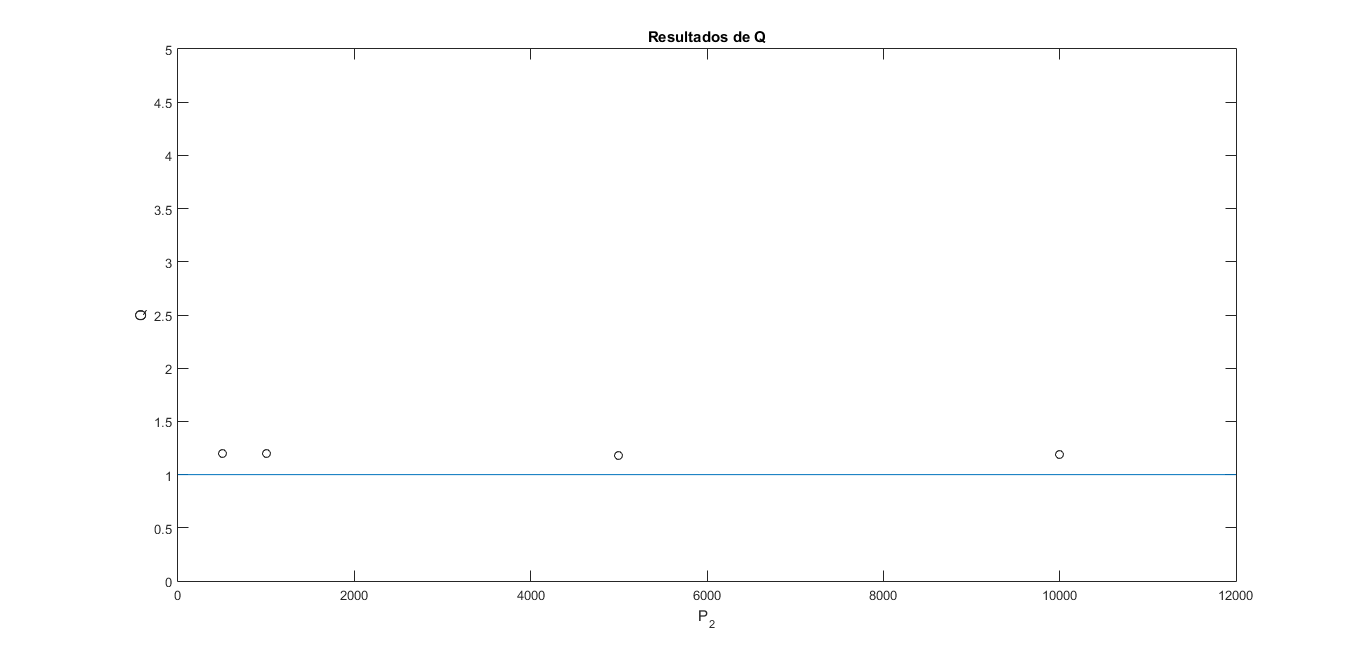
\includegraphics[angle=0,width=1\textwidth]{RelacaoQP2TT.png}
     \captionof{figure}{Comparação experiência/teoria da relação entre $K$ medido em $T_1$ e o valor de $P_2$.}
     \label{fig:RelacaoQP2TT}
     \end{center}

A estimação de $Q$ a partir dos dados experimentais revela erros relativos entre $18\%$ e $20\%$, o que já não pode ser considerado aceitável. Contudo, tomando em consideração a forma como foram obtidos os valores de $Q$ apresentados, não é difícil encontrar factores que possam ter promovido esta falta de exactidão. Em primeiro lugar, não foram feitas medidas suficientes na região de frequências passante, o que implica uma interpolação posterior mais fraca e menos concordante com o sistema real observado. De facto, em frequência próximas da dos pólos do sistema as razões de amplitude entrada-saída variam rapidamente e, dessa forma, uma má estimação em torno do pico de ganho máximo é facilmente obtida. Este factor induz também, obviamente, erro na estimação de $\omega_p$. Em segundo lugar e em consequência do primeiro factor, uma interpolação por \textit{splines} não consegue compensar a falta de pontos para interpolar e \emph{desenhar} o pico esperado, ao passo que uma interpolação com uma função racional poderia, com um número de pontos mais elevado, ter estimado um pico de ganho máximo com um aspecto mais próximo do teórico.\\
Por outro lado, a estimação de $Q$ revela ser bastante precisa, embora que inexacta. De facto, os resultados de $Q$ apresentam uma variância de $3.67\%$. Ora, se a falta de exactidão pode, por um lado, ser explicada pelo método utilizado na interpolação, a elevada precisão revela, por outro, que talvez haja outro factor, comum a todas as medições, a induzir erro na medição. Ou seja, a precisão obtida indica que talvez o factor de qualidade do sistema real observado não seja, já por si, igual ao teórico.

\chapter{Conclusões}

Nesta atividade laboratorial foi possível aos alunos familiarizarem-se com diagramas de fluxo de sinal e relacioná-los com circuitos elétricos e montarem os mesmos nas \textit{breadboards} com recurso a circuitos integrados, resistências e condensadores.\\
Estes circuitos montados são filtros de frequência (passa-banda, passa-alto e passa-baixo) com ganhos bastante razoáveis.
Os resultados experimentais revelaram nas duas experiências não serem totalmente concordantes com os teóricos revelando os obstáculos de passar a teoria à prática. Mesmo com tentativas de ajuste não é fácil obter os valores tão precisos como na teoria.\\
É de notar que os filtros não estão limitados só na frequência, mas também na amplitude do sinal e, como tal os filtros têm um funcionamento menos fiável para amplitudes muito baixas ou para amplitudes muito altas (nomeadamente com a saturação dos Amplificadores Operacionais).

\end{document}